\section{Contents of Audit Files}

As well as storing the hash representation of application control-flow, the proposed solution will also be able to offer the ability to store additional data, bound to the historic control-flow. This additional data will use useful for proving the state of the application execution as well as the operating state of the embedded system itself.

A historic chain of audit files will be built up by including hashes of the previous file in each audit file, with the first also containing the initial attestation report. The resulting audit files will either be signed or have an HMAC created for them (with digital signatures being the preferable method due to them providing non-repudiation). The audit file may also be encrypted depending on the security requirements. 

\subsubsection*{Execution Variables}

The solution will implement a function where variables can be stored alongside the representation of control-flow happening at that moment in time. Through the addition of an API, the solution will enable a software developer to perform an assert (where data is sent to secure world). When an assert is triggered, the hash representation of the control-flow will be taken from the measurement engine and stored along with the variables included in the assert.

The addition of this feature will be useful for proving that, as well as the application executing as it should (by following its CFG), the variables used within important functions are as they are expected to be.

\subsubsection*{Concurrently Running Processes}

When implemented with a multi-tasking enabled OS, the solution will present an option within the API to store a record of processes also running on the device  at the same time as the control-flow hash. When triggered, the process will query the running processes from the OS and extract useful information about each process, including process name and file location.

This feature will provide an indication of the state of the device and should capture the existence of other processes which may interfere with the audited application. 

\begin{figure}
  \centering
  \vspace*{0.5in}
  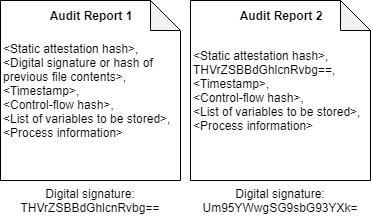
\includegraphics[scale=0.5]{Files.png}
  \caption{The contents of control-flow audit files}
  \label{fig:auditFiles}
\end{figure}
